\chapter{Models}\label{models}

\section{Overview}\label{models:overview}

Chapters~\ref{ps} through~\ref{nls} presented the different
``iterators'' (or methods) available in Dakota.  An iterator iterates
on a model in order to map a set of variables into a set of responses.
This model may involve a simple mapping involving a single interface,
or it may involve recursions using sub-iterators and sub-models.  These
recursion capabilities were developed in order to provide mechanisms
for ``nesting,'' ``layering,'' and ``recasting'' of software
components, which allows the use of these components as building
blocks to accomplish more sophisticated studies, such as
surrogate-based optimization or optimization under uncertainty.  In a
nested relationship, a sub-iterator is executed using its sub-model
for every evaluation of the nested model.  In a layered relationship,
on the other hand, sub-iterators and sub-models are used only for
periodic updates and verifications.  And in a recast relationship, the
input variable and output response definitions in a sub-model are
reformulated in order to support new problem definitions.  In each of
these cases, the sub-model is of arbitrary type, such that model
recursions can be chained together in as long of a sequence as needed
(e.g., layered containing nested contained layered containing single
in Section~\ref{adv_models:ouu:sb}).  Figure~\ref{model:hier} displays
the model class hierarchy from the Dakota Developers
Manual~\cite{DevMan}, with derived classes for single models, nested
models, recast models, and two types of surrogate models: data fit and
hierarchical/multifidelity.  A third type of derived surrogate model
supporting reduced-order models (ROM) is planned for future releases.

\begin{figure}
  \centering 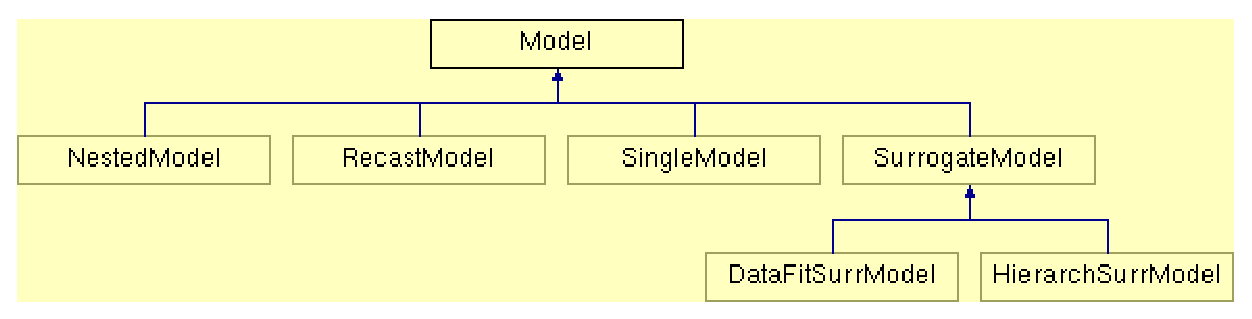
\includegraphics[scale=0.65]{images/classDakota_1_1Model}
  \caption{The Dakota model class hierarchy.}  \label{model:hier}
\end{figure}

Section~\ref{models:single} describes single models,
Section~\ref{models:recast} describes recast models,
Section~\ref{models:surrogate} describes surrogate models of various
types, Section~\ref{models:nested} describes nested models, Section
~\ref{models:randomfield} describes random field models, and Section
~\ref{models:subspace} describes active subspace models.  Finally,
Chapter~\ref{adv_models} presents a number of advanced examples
demonstrating these model recursions.

\section{Single Models}\label{models:single}

The single model is the simplest model type.  It uses a single
interface instance (see Chapter~\ref{interfaces}) to map variables
(see Chapter~\ref{variables}) into responses (see
Chapter~\ref{responses}).  There is no recursion in this case.  Refer
to the Models chapter in the Dakota Reference Manual~\cite{RefMan} for
additional information on the single model specification.

\section{Recast Models}\label{models:recast}

The recast model is not directly visible to the user within the input
specification.  Rather, it is used ``behind the scenes'' to recast the
inputs and outputs of a sub-model for the purposes of reformulating
the problem posed to an iterator.  Examples include variable and
response scaling (see Section~\ref{opt:additional:scaling}),
transformations of uncertain variables and associated response
derivatives to employ standardized random variables (see
Sections~\ref{uq:reliability} and~\ref{uq:expansion}), multiobjective
optimization (see Section~\ref{opt:additional:multiobjective}), merit
functions (see Section~\ref{adv_meth:sbm:sblm}), and expected
improvement/feasibility (see Sections~\ref{opt:methods:gradientfree:global}
and~\ref{uq:reliability:global}).  Refer to the Dakota Developers
Manual~\cite{DevMan} for additional details on the mechanics of
recasting problem formulations.

\section{Surrogate Models}\label{models:surrogate}

Surrogate models are inexpensive approximate models that are intended
to capture the salient features of an expensive high-fidelity model.
They can be used to explore the variations in response quantities over
regions of the parameter space, or they can serve as inexpensive
stand-ins for optimization or uncertainty quantification studies (see,
for example, the surrogate-based optimization methods in
Section~\ref{adv_meth:sbm}).  Surrogate models supported in Dakota can be
categorized into three types: data fits, multifidelity, and
reduced-order model surrogates.  An overview and discussion of
surrogate correction is provided here, with details following.

\subsection{Overview of Surrogate Types}


Data fitting methods involve construction of an approximation or
surrogate model using data (response values, gradients, and Hessians)
generated from the original truth model.  Data fit methods can be
further categorized as local, multipoint, and global approximation
techniques, based on the number of points used in generating the data
fit.  Local methods involve response data from a single point in
parameter space.  Available local techniques currently include:
  
\emph{Known Issue: When using discrete variables, there have been
  sometimes significant differences in data fit surrogate behavior
  observed across computing platforms in some cases.  The cause has
  not yet been fully diagnosed and is currently under investigation.
  In addition, guidance on appropriate construction and use of
  surrogates with discrete variables is under development.  In the
  meantime, users should therefore be aware that there is a risk of
  inaccurate results when using surrogates with discrete variables.}

\textbf{Taylor Series Expansion}: This is a local first-order or
second-order expansion centered at a single point in the parameter space.

Multipoint approximations involve response data from two or more
points in parameter space, often involving the current and previous
iterates of a minimization algorithm.  Available techniques currently
include:

\textbf{TANA-3}: This multipoint approximation uses a two-point
exponential approximation~\cite{Xu98,Fad90} built with response value
and gradient information from the current and previous iterates.

Global methods, often referred to as \emph{response surface methods},
involve many points spread over the parameter ranges of interest.
These surface fitting methods work in conjunction with the sampling
methods and design of experiments methods described in
Sections~\ref{uq:sampling} and ~\ref{dace:background}.

\textbf{Polynomial Regression}: First-order (linear), second-order
(quadratic), and third-order (cubic) polynomial response surfaces
computed using linear least squares regression methods. Note: there is
currently no use of forward- or backward-stepping regression methods
to eliminate unnecessary terms from the polynomial model.

\textbf{Gaussian Process (GP) or Kriging Interpolation}
Dakota contains two implementations of Gaussian process, also known as 
Kriging ~\cite{Giu98}, spatial interpolation.  One of these resides in 
the Surfpack sub-package of Dakota, the other resides in Dakota itself.
Both versions use the Gaussian correlation function with parameters that
are selected by Maximum Likelihood Estimation (MLE). This correlation 
function results in a response surface that is $C^\infty$-continuous.
Prior to Dakota 5.2, the Surfpack GP was referred to as the ``Kriging'' 
model and the Dakota version was labeled as the ``Gaussian Process.''  
These terms are now used interchangeably.  As of Dakota 5.2,the 
Surfpack GP is used by default.  For now the user still has the option 
to select the Dakota GP, but the Dakota GP is deprecated and will be 
removed in a future release.
\begin{itemize}
\item \textbf{Surfpack GP}: Ill-conditioning due to a poorly spaced sample 
      design is handled by discarding points that contribute the least 
      unique information to the correlation matrix.  Therefore, the points 
      that are discarded are the ones that are easiest to predict.  The 
      resulting surface will exactly interpolate the data values at the 
      retained points but is not guaranteed to interpolate the discarded 
      points.
\item \textbf{Dakota GP}: Ill-conditioning is handled by adding a jitter 
      term or ``nugget'' to diagonal elements of the correlation matrix. 
      When this happens, the Dakota GP may not exactly interpolate the 
      data values.
\end{itemize}

\textbf{Artificial Neural Networks}: An implementation of the
stochastic layered perceptron neural network developed by Prof. D. C.
Zimmerman of the University of Houston~\cite{Zim96}. This neural network
method is intended to have a lower training (fitting) cost than
typical back-propagation neural networks.

\textbf{Multivariate Adaptive Regression Splines (MARS)}: Software
developed by Prof. J. H. Friedman of Stanford University~\cite{Fri91}.
The MARS method creates a $C^2$-continuous patchwork of splines in the
parameter space.

\textbf{Radial Basis Functions (RBF)}:  Radial basis functions are 
functions whose value typically depends on the distance from a center point, 
called the centroid.  The surrogate model approximation is constructed
as the weighted sum of individual radial basis functions. 

\textbf{Moving Least Squares (MLS)}: Moving Least Squares can be 
considered a more specialized version of linear regression models.
MLS is a weighted least squares approach where the weighting is 
``moved'' or recalculated for every new point where 
a prediction is desired.~\cite{Nea04} 

\textbf{Piecewise Decomposition Option for Global Surrogates}: Typically, the previous regression techniques use all available sample points to approximate the underlying function anywhere in the domain. An alternative option is to use piecewise decomposition to locally approximate the function at some point using a few sample points from its neighborhood. This option currently supports Polynomial Regression, Gaussian Process (GP) Interpolation, and Radial Basis Functions (RBF) Regression. It requires a decomposition cell type (currently set to be Voronoi cells), an optional number of support layers of neighbors, and optional discontinuity detection parameters (jump/gradient).   

%\textbf{Orthogonal Polynomials}: This technique involves the use of
%multivariate orthogonal polynomials as a global basis for surrogate
%modeling.  These multivariate polynomials are constructed as a product
%of particular univariate orthogonal polynomials, including Hermite,
%Legendre, Laguerre, Jacobi, and generalized Laguerre polynomials,
%which are defined as functions of standard normal, standard uniform,
%standard exponential, standard beta, and standard gamma random
%variables, respectively.  Given the probabilistic interpretation of
%the approximation variables, this data fit is primarily used for
%uncertainty quantification, and in particular, polynomial chaos
%expansions.

In addition to data fit surrogates, Dakota supports multifidelity 
and reduced-order model approximations:

\textbf{Multifidelity Surrogates}: Multifidelity modeling involves the
use of a low-fidelity physics-based model as a surrogate for the
original high-fidelity model.  The low-fidelity model typically
involves a coarser mesh, looser convergence tolerances, reduced
element order, or omitted physics.  It is a separate model in its own
right and does not require data from the high-fidelity model for
construction.  Rather, the primary need for high-fidelity evaluations
is for defining correction functions that are applied to the
low-fidelity results.

\textbf{Reduced Order Models}: A reduced-order model (ROM) is
mathematically derived from a high-fidelity model using the technique
of Galerkin projection.  By computing a set of basis functions (e.g.,
eigenmodes, left singular vectors) that capture the principal dynamics
of a system, the original high-order system can be projected to a much
smaller system, of the size of the number of retained basis functions.

\subsection{Correction Approaches}

Each of the surrogate model types supports the use of correction
factors that improve the local accuracy of the surrogate models. The
correction factors force the surrogate models to match the true
function values and possibly true function derivatives at the center
point of each trust region. Currently, Dakota supports either zeroth-,
first-, or second-order accurate correction methods, each of which can
be applied using either an additive, multiplicative, or combined
correction function. For each of these correction approaches, the
correction is applied to the surrogate model and the corrected model
is then interfaced with whatever algorithm is being employed.  The
default behavior is that no correction factor is applied.

The simplest correction approaches are those that enforce consistency
in function values between the surrogate and original models at a
single point in parameter space through use of a simple scalar offset
or scaling applied to the surrogate model.  First-order corrections
such as the first-order multiplicative correction (also known as beta
correction~\cite{Cha93}) and the first-order additive
correction~\cite{Lew00} also enforce consistency in the gradients and
provide a much more substantial correction capability that is
sufficient for ensuring provable convergence in SBO algorithms (see
Section~\ref{adv_meth:sbm:sblm}).  SBO convergence rates can be further
accelerated through the use of second-order corrections which also
enforce consistency in the Hessians~\cite{Eld04}, where the
second-order information may involve analytic, finite-difference, or
quasi-Newton Hessians.

Correcting surrogate models with additive corrections involves
\begin{equation}
\hat{f_{hi_{\alpha}}}({\bf x}) = f_{lo}({\bf x}) + \alpha({\bf x}) 
\label{eq:correct_val_add}
\end{equation}
where multifidelity notation has been adopted for clarity.  For
multiplicative approaches, corrections take the form
\begin{equation}
\hat{f_{hi_{\beta}}}({\bf x}) = f_{lo}({\bf x}) \beta({\bf x})
\label{eq:correct_val_mult}
\end{equation}
where, for local corrections, $\alpha({\bf x})$ and $\beta({\bf x})$
are first or second-order Taylor series approximations to the exact
correction functions:
\begin{eqnarray}
\alpha({\bf x}) & = & A({\bf x_c}) + \nabla A({\bf x_c})^T 
({\bf x} - {\bf x_c}) + \frac{1}{2} ({\bf x} - {\bf x_c})^T 
\nabla^2 A({\bf x_c}) ({\bf x} - {\bf x_c}) \label{eq:taylor_a} \\
\beta({\bf x})  & = & B({\bf x_c}) + \nabla B({\bf x_c})^T 
({\bf x} - {\bf x_c}) + \frac{1}{2} ({\bf x} - {\bf x_c})^T \nabla^2 
B({\bf x_c}) ({\bf x} - {\bf x_c}) \label{eq:taylor_b}
\end{eqnarray}
where the exact correction functions are
\begin{eqnarray}
A({\bf x}) & = & f_{hi}({\bf x}) - f_{lo}({\bf x})       \label{eq:exact_A} \\
B({\bf x}) & = & \frac{f_{hi}({\bf x})}{f_{lo}({\bf x})} \label{eq:exact_B}
\end{eqnarray}
Refer to \cite{Eld04} for additional details on the derivations.

A combination of additive and multiplicative corrections can provide
for additional flexibility in minimizing the impact of the correction
away from the trust region center.  In other words, both additive and
multiplicative corrections can satisfy local consistency, but through
the combination, global accuracy can be addressed as well.  This
involves a convex combination of the additive and multiplicative
corrections:
\begin{equation}
\hat{f_{hi_{\gamma}}}({\bf x}) = \gamma \hat{f_{hi_{\alpha}}}({\bf x}) +
(1 - \gamma) \hat{f_{hi_{\beta}}}({\bf x}) \label{eq:combined_form}
\end{equation}
where $\gamma$ is calculated to satisfy an additional matching
condition, such as matching values at the previous design iterate.

%It should be noted that in both first order correction methods, the
%function $\hat{f}(x)$ matches the function value and gradients of
%$f_{t}(x)$ at $x=x_{c}$. This property is necessary in proving that
%the first order-corrected SBO algorithms are provably convergent to a
%local minimum of $f_{t}(x)$.  However, the first order correction
%methods are significantly more expensive than the zeroth order
%correction methods, since the first order methods require computing
%both $\nabla f_{t}(x_{c})$ and $\nabla f_{s}(x_{c})$.  When the SBO
%strategy is used with either of the zeroth order correction methods,
%or with no correction method, convergence is not guaranteed to a local
%minimum of $f_{t}(x)$. That is, the SBO strategy becomes a heuristic
%optimization algorithm. From a mathematical point of view this is
%undesirable, but as a practical matter, the heuristic variants of SBO
%are often effective in finding local minima.

%\emph{Usage guidelines:}
%\begin{itemize}
%\item Both the \texttt{additive zeroth\_order} and
%  \texttt{multiplicative zeroth\_order} correction methods are
%  ``free'' since they use values of $f_{t}(x_{c})$ that are normally
%  computed by the SBO strategy.
%
%\item The use of either the \texttt{additive first\_order} method or
%  the \texttt{multiplicative first\_order} method does not necessarily
%  improve the rate of convergence of the SBO algorithm.
%
%\item When using the first order correction methods, the
%  \texttt{TRUE\_FCN\_GRAD} response keywords must be modified (see
%  bottom of Figure~\ref{sbm:sblm_rosen}) to allow either analytic or
%  numerical gradients to be computed. This provides the gradient data
%  needed to compute the correction function.
%
%\item For many computationally expensive engineering optimization
%  problems, gradients often are too expensive to obtain or are
%  discontinuous (or may not exist at all). In such cases the heuristic
%  SBO algorithm has been an effective approach at identifying optimal
%  designs~\cite{Giu02}.
%\end{itemize}

\subsection{Data Fit Surrogate Models}\label{models:surrogate:datafit}

A surrogate of the {\em data fit} type is a non-physics-based
approximation typically involving interpolation or regression of a set
of data generated from the original model.  Data fit surrogates can be
further characterized by the number of data points used in the fit,
where a local approximation (e.g., first or second-order Taylor
series) uses data from a single point, a multipoint approximation
(e.g., two-point exponential approximations (TPEA) or two-point
adaptive nonlinearity approximations (TANA)) uses a small number of
data points often drawn from the previous iterates of a particular
algorithm, and a global approximation (e.g., polynomial response
surfaces, kriging/gaussian\_process, neural networks, radial basis 
functions, splines)
uses a set of data points distributed over the domain of interest,
often generated using a design of computer experiments.

Dakota contains several types of surface fitting methods that can be
used with optimization and uncertainty quantification methods and
strategies such as surrogate-based optimization and optimization under
uncertainty. These are: polynomial models (linear, quadratic, and
cubic), first-order Taylor series expansion, kriging spatial
interpolation, artificial neural networks, multivariate adaptive
regression splines, radial basis functions, and moving least squares. 
With the exception of Taylor series methods, all of the above methods 
listed in the previous sentence are accessed in Dakota through the 
Surfpack library.  All of these surface fitting methods can be
applied to problems having an arbitrary number of design parameters.
However, surface fitting methods usually are practical only for
problems where there are a small number of parameters (e.g., a maximum
of somewhere in the range of 30-50 design parameters). The
mathematical models created by surface fitting methods have a variety
of names in the engineering community. These include surrogate models,
meta-models, approximation models, and response surfaces. For this
manual, the terms surface fit model and surrogate model are used.

The data fitting methods in Dakota include software developed by
Sandia researchers and by various researchers in the academic
community.

\subsubsection{Procedures for Surface Fitting}\label{models:surf:procedures}

The surface fitting process consists of three steps: (1) selection of
a set of design points, (2) evaluation of the true response quantities
(e.g., from a user-supplied simulation code) at these design points,
and (3) using the response data to solve for the unknown coefficients
(e.g., polynomial coefficients, neural network weights, kriging
correlation factors) in the surface fit model. In cases where there is
more than one response quantity (e.g., an objective function plus one
or more constraints), then a separate surface is built for each
response quantity. Currently, most surface fit models are built using
only 0$^{\mathrm{th}}$-order information (function values only),
although extensions to using higher-order information (gradients and
Hessians) are possible, and the Kriging model does allow construction
for gradient data. Each surface fitting method employs a different
numerical method for computing its internal coefficients. For example,
the polynomial surface uses a least-squares approach that employs a
singular value decomposition to compute the polynomial coefficients,
whereas the kriging surface uses Maximum Likelihood Estimation to
compute its correlation coefficients. More information on the
numerical methods used in the surface fitting codes is provided in the
Dakota Developers Manual~\cite{DevMan}.

The set of design points that is used to construct a surface fit model
is generated using either the DDACE software package~\cite{TonXX} or
the LHS software package~\cite{Ima84}. These packages provide a
variety of sampling methods including Monte Carlo (random) sampling,
Latin hypercube sampling, orthogonal array sampling, central composite
design sampling, and Box-Behnken sampling. More information on these
software packages is provided in Chapter~\ref{dace}.  Optionally, the
quality of a surrogate model can be assessed with surrogate metrics or
diagnostics as described in Section~\ref{models:surf:diagnostics}.

\subsubsection{Taylor Series}\label{models:surf:taylor}

The Taylor series model is purely a local approximation method. That
is, it provides local trends in the vicinity of a single point in
parameter space. The first-order Taylor series expansion is:
\begin{equation}
\hat{f}({\bf x}) \approx f({\bf x}_0) + \nabla_{\bf x} f({\bf x}_0)^T 
({\bf x} - {\bf x}_0) \label{eq:taylor1}
\end{equation}
and the second-order expansion is:
\begin{equation}
\hat{f}({\bf x}) \approx f({\bf x}_0) + \nabla_{\bf x} f({\bf x}_0)^T 
({\bf x} - {\bf x}_0) + \frac{1}{2} ({\bf x} - {\bf x}_0)^T 
\nabla^2_{\bf x} f({\bf x}_0) ({\bf x} - {\bf x}_0) \label{eq:taylor2}
\end{equation}

where ${\bf x}_0$ is the expansion point in $n$-dimensional parameter
space and $f({\bf x}_0)$, $\nabla_{\bf x} f({\bf x}_0)$, and
$\nabla^2_{\bf x} f({\bf x}_0)$ are the computed response value,
gradient, and Hessian at the expansion point, respectively.  As
dictated by the responses specification used in building the local
surrogate, the gradient may be analytic or numerical and the Hessian
may be analytic, numerical, or based on quasi-Newton secant updates.

In general, the Taylor series model is accurate only in the region of
parameter space that is close to ${\bf x}_0$ . While the accuracy is
limited, the first-order Taylor series model reproduces the correct
value and gradient at the point $\mathbf{x}_{0}$, and the second-order
Taylor series model reproduces the correct value, gradient, and
Hessian. This consistency is useful in provably-convergent
surrogate-based optimization. The other surface fitting methods do not
use gradient information directly in their models, and these methods
rely on an external correction procedure in order to satisfy the
consistency requirements of provably-convergent SBO.

\subsubsection{Two Point Adaptive Nonlinearity Approximation}\label{models:surf:tana}

The TANA-3 method~\cite{Xu98} is a multipoint approximation method
based on the two point exponential approximation~\cite{Fad90}. This
approach involves a Taylor series approximation in intermediate
variables where the powers used for the intermediate variables are
selected to match information at the current and previous expansion
points.  The form of the TANA model is:

\begin{equation}
\hat{f}({\bf x}) \approx f({\bf x}_2) + \sum_{i=1}^n 
\frac{\partial f}{\partial x_i}({\bf x}_2) \frac{x_{i,2}^{1-p_i}}{p_i} 
(x_i^{p_i} - x_{i,2}^{p_i}) + \frac{1}{2} \epsilon({\bf x}) \sum_{i=1}^n 
(x_i^{p_i} - x_{i,2}^{p_i})^2 \label{eq:tana_f}
\end{equation}

where $n$ is the number of variables and:

\begin{eqnarray}
p_i & = & 1 + \ln \left[ \frac{\frac{\partial f}{\partial x_i}({\bf x}_1)}
{\frac{\partial f}{\partial x_i}({\bf x}_2)} \right] \left/ 
\ln \left[ \frac{x_{i,1}}{x_{i,2}} \right] \right. \label{eq:tana_pi} \\
\epsilon({\bf x}) & = & \frac{H}{\sum_{i=1}^n (x_i^{p_i} - x_{i,1}^{p_i})^2 + 
\sum_{i=1}^n (x_i^{p_i} - x_{i,2}^{p_i})^2} \label{eq:tana_eps} \\
H & = & 2 \left[ f({\bf x}_1) - f({\bf x}_2) - \sum_{i=1}^n 
\frac{\partial f}{\partial x_i}({\bf x}_2) \frac{x_{i,2}^{1-p_i}}{p_i} 
(x_{i,1}^{p_i} - x_{i,2}^{p_i}) \right] \label{eq:tana_H}
\end{eqnarray}

and ${\bf x}_2$ and ${\bf x}_1$ are the current and previous expansion
points.  Prior to the availability of two expansion points, a
first-order Taylor series is used.

\subsubsection{Linear, Quadratic, and Cubic Polynomial Models}\label{models:surf:polynomial}

Linear, quadratic, and cubic polynomial models are available in
Dakota. The form of the linear polynomial model is

\begin{equation}
  \hat{f}(\mathbf{x}) \approx c_{0}+\sum_{i=1}^{n}c_{i}x_{i}
  \label{models:surf:equation01}
\end{equation}

the form of the quadratic polynomial model is:

\begin{equation}
  \hat{f}(\mathbf{x}) \approx c_{0}+\sum_{i=1}^{n}c_{i}x_{i}
  +\sum_{i=1}^{n}\sum_{j \ge i}^{n}c_{ij}x_{i}x_{j}
  \label{models:surf:equation02}
\end{equation}

and the form of the cubic polynomial model is:

\begin{equation}
  \hat{f}(\mathbf{x}) \approx c_{0}+\sum_{i=1}^{n}c_{i}x_{i}
  +\sum_{i=1}^{n}\sum_{j \ge i}^{n}c_{ij}x_{i}x_{j}
  +\sum_{i=1}^{n}\sum_{j \ge i}^{n}\sum_{k \ge j}^{n}
  c_{ijk}x_{i}x_{j}x_{k}
  \label{models:surf:equation03}
\end{equation}

In all of the polynomial models, $\hat{f}(\mathbf{x})$ is the response
of the polynomial model; the $x_{i},x_{j},x_{k}$ terms are the
components of the $n$-dimensional design parameter values; the $c_{0}$
, $c_{i}$ , $c_{ij}$ , $c_{ijk} $ terms are the polynomial
coefficients, and $n$ is the number of design parameters.  The number
of coefficients, $n_{c}$, depends on the order of polynomial model and
the number of design parameters. For the linear polynomial:

\begin{equation}
  n_{c_{linear}}=n+1
  \label{models:surf:equation04}
\end{equation}

for the quadratic polynomial:

\begin{equation}
  n_{c_{quad}}=\frac{(n+1)(n+2)}{2}
  \label{models:surf:equation05}
\end{equation}

and for the cubic polynomial:

\begin{equation}
  n_{c_{cubic}}=\frac{(n^{3}+6 n^{2}+11 n+6)}{6}
  \label{models:surf:equation06}
\end{equation}

There must be at least $n_{c}$ data samples in order to form a fully
determined linear system and solve for the polynomial coefficients. For
discrete design variables, a further requirement for a well-posed
problem is for the number of distinct values that each discrete
variable can take must be greater than the order of polynomial model
(by at least one level). For the special case involving anisotropy in
which the degree can be specified differently per dimension, the number
of values for each discrete variable needs to be greater than the 
corresponding order along the respective dimension. In Dakota, a
least-squares approach involving a singular value decomposition
numerical method is applied to solve the linear system.

The utility of the polynomial models stems from two sources: (1) over
a small portion of the parameter space, a low-order polynomial model
is often an accurate approximation to the true data trends, and (2)
the least-squares procedure provides a surface fit that smooths out
noise in the data. For this reason, the surrogate-based optimization
approach often is successful when using polynomial models,
particularly quadratic models. However, a polynomial surface fit may
not be the best choice for modeling data trends over the entire
parameter space, unless it is known a priori that the true data trends
are close to linear, quadratic, or cubic. See~\cite{Mye95} for more
information on polynomial models.

This surrogate model supports the domain decomposition option, further explained in~\ref{models:surf:piecewise_decomp}.

\subsubsection{Kriging/Gaussian-Process Spatial Interpolation Models}
\label{models:surf:kriging}
In the current release of Dakota, we have two versions of spatial interpolation 
models. One is located in Dakota itself and the other in the Surfpack subpackage 
of Dakota which can be compiled in a stand alone mode.  These models
are denoted as \texttt{kriging dakota} and \texttt{kriging surfpack} or 
as \texttt{gaussian\_process dakota} and 
\texttt{gaussian\_process surfpack}.  In Dakota releases prior to 5.2, the 
\texttt{dakota} version was referred to as the \texttt{gaussian\_process} 
model while the \texttt{surfpack} version was referred to as the 
\texttt{kriging} model.  As of Dakota 5.2, specifying only
\texttt{gaussian\_process} or \texttt{kriging} will default to the
\texttt{surfpack} version in all contexts except Bayesian calibration.  
For now, both versions are supported but the \texttt{dakota} version is 
deprecated and intended to be removed in a future release.  The two 
\texttt{kriging} or \texttt{gaussian\_process} models are very similar: 
the differences between them are explained in more detail below.

The Kriging, also known as Gaussian process (GP), method uses techniques 
developed in the geostatistics and spatial statistics communities 
(~\cite{Cre91},~\cite{Koe96}) to produce smooth surface fit models of the 
response values from a set of data points.  The number of times the 
fitted surface is differentiable will depend on the correlation function 
that is used.  Currently, the Gaussian correlation function is the only 
option for either version included in Dakota; this makes the GP model 
$C^{\infty}$-continuous.  The form of the GP model is

\begin{equation}
  \hat{f}(\underline{x}) \approx \underline{g}(\underline{x})^T\underline{\beta} +
  \underline{r}(\underline{x})^{T}\underline{\underline{R}}^{-1}(\underline{f}-\underline{\underline{G}}\ \underline{\beta})
  \label{models:surf:equation08}
\end{equation}

where $\underline{x}$ is the current point in $n$-dimensional parameter
space; $\underline{g}(\underline{x})$ is the vector of trend basis 
functions evaluated at $\underline{x}$; $\underline{\beta}$ is a vector
containing the generalized least squares estimates of the trend basis 
function coefficients; $\underline{r}(\underline{x})$ is the correlation 
vector of terms between $\underline{x}$ and the data points;
$\underline{\underline{R}}$ is the correlation matrix for all of the 
data points; $\underline{f}$ is the vector of response values; and 
$\underline{\underline{G}}$ is the matrix containing the trend basis 
functions evaluated at all data points.  The terms in the correlation 
vector and matrix are computed using a Gaussian correlation function 
and are dependent on an $n$-dimensional vector of correlation parameters,
$\underline{\theta} = \{\theta_{1},\ldots,\theta_{n}\}^T$. By default, 
Dakota determines the value of $\underline{\theta}$ using a Maximum
Likelihood Estimation (MLE) procedure.  However, the user can also opt 
to manually set them in the \texttt{gaussian\_process surfpack}
model by specifying a vector of correlation lengths, 
$\underline{l}=\{l_{1},\ldots,l_{n}\}^T$ where 
$\theta_i=1/(2 l_i^2)$. This definition of correlation lengths makes 
their effect on the GP model's behavior directly analogous to the 
role played by the standard deviation in a normal (a.k.a. Gaussian) 
distribution.  In the \texttt{gaussian\_process surpack} model, we used 
this analogy to define a small feasible region in which to search for 
correlation lengths.  This region should (almost) always contain some 
correlation matrices that are well conditioned and some that are optimal, 
or at least near optimal. More details on Kriging/GP models may be 
found in~\cite{Giu98}.

Since a GP has a hyper-parametric error model, it can be used 
to model surfaces with slope discontinuities along with multiple 
local minima and maxima. GP interpolation is useful for both 
SBO and OUU, as well as for studying the global response value trends 
in the parameter space. This surface fitting method needs a 
minimum number of design points equal to the sum of the number of 
basis functions and the number of dimensions, $n$, but it is 
recommended to use at least double this amount.
%$n_{c_{quad}}$ design points when possible (refer to
%Section~\ref{models:surf:polynomial} for $n_{c}$ definitions).

The GP model is guaranteed to pass through all of the response 
data values that are used to construct the model. Generally, this is a
desirable feature. However, if there is considerable numerical noise
in the response data, then a surface fitting method that provides some
data smoothing (e.g., quadratic polynomial, MARS) may be a better
choice for SBO and OUU applications. Another feature of the GP
model is that the predicted response values, $\hat{f}(\underline{x})$,
decay to the trend function, 
$\underline{g}(\underline{x})^T\underline{\beta}$, when $\underline{x}$ 
is far from any of the data points from which the GP model was 
constructed (i.e., when the model is used for extrapolation). 

As mentioned above, there are two \texttt{gaussian\_process} models 
in Dakota, the \texttt{surfpack} version and the \texttt{dakota}
version.  More details on the \texttt{gaussian\_process dakota}
model can be found in~\cite{McF08}. The differences between these 
models are as follows: 

\begin{itemize}
\item Trend Function:  The GP models incorporate a parametric trend 
      function whose purpose is to capture large-scale variations. In 
      both models, the trend function can be a constant, linear,or 
      reduced quadratic (main effects only, no interaction terms) 
      polynomial.  This is specified by the keyword \texttt{trend}
      followed by one of \texttt{constant}, \texttt{linear}, or 
      \texttt{reduced\_quadratic} (in Dakota 5.0 and earlier, the reduced 
      quadratic option for the \texttt{dakota} version was selected using 
      the keyword, \texttt{quadratic}). The \\
      \texttt{gaussian\_process surfpack} model has the additional option 
      of a full (i.e. it includes interaction terms) quadratic polynomial; 
      this is accessed by following the \texttt{trend} keyword with 
      \texttt{quadratic}.
\item Correlation Parameter Determination: Both of the 
      \texttt{gaussian\_process} models use a Maximum Likelihood Estimation 
      (MLE) approach to find the optimal values of the hyper-parameters 
      governing the mean and correlation functions. By default both models 
      use the global optimization method called DIRECT, although they search 
      regions with different extents. For the 
      \texttt{gaussian\_process dakota} model, DIRECT is the only option.  
      The \texttt{gaussian\_process surfpack} model has several options for 
      the optimization method used.  These are specified by the 
      \texttt{optimization\_method} keyword followed by one of these strings:
      \begin{itemize}
      \item \texttt{'global'} which uses the default DIRECT optimizer,
      \item \texttt{'local'} which uses the CONMIN optimizer,
      \item \texttt{'sampling'} which generates several random guesses and 
            picks the candidate with greatest likelihood, and
      \item \texttt{'none'} 
      \end{itemize} 
      The \texttt{'none'} option, and the starting location of the 
      \texttt{'local'} optimization, default to the center, in 
      log(correlation length) scale, of the small feasible region.  
      However, these can also be user specified with the 
      \texttt{correlation\_lengths} keyword followed by a list of $n$ real 
      numbers.  The total number of evaluations of the 
      \texttt{gaussian\_process surfpack} model's likelihood function can 
      be controlled using the \texttt{max\_trials} keyword followed by a 
      positive integer.  Note that we have found the \texttt{'global'} 
      optimization method to be the most robust.
\item Ill-conditioning.  One of the major problems in determining 
      the governing values for a Gaussian process or Kriging model is 
      the fact that the correlation matrix can easily become 
      ill-conditioned when there are too many input points close together.
      Since the predictions from the Gaussian process model involve 
      inverting the correlation matrix, ill-conditioning can lead to poor 
      predictive capability and should be avoided. The 
      \texttt{gaussian\_process surfpack} model defines a small feasible 
      search region for correlation lengths, which should (almost) always 
      contain some well conditioned correlation matrices. In Dakota 5.1, 
      the \texttt{kriging} (now \texttt{gaussian\_process surfpack} or
      \texttt{kriging surfpack}) model avoided 
      ill-conditioning by explicitly excluding poorly conditioned 
      $\underline{\underline{R}}$ from consideration on the basis of their 
      having a large (estimate of) condition number; this constraint acted 
      to decrease the size of admissible correlation lengths.  Note that a
      sufficiently bad sample design could require correlation lengths to 
      be so short that any interpolatory Kriging/GP model would become 
      inept at extrapolation and interpolation. \\ \\
      The \texttt{gaussian\_process dakota} model has two features to 
      overcome ill-conditioning.  The first is that the algorithm will 
      add a small amount of noise to the diagonal elements of the matrix 
      (this is often referred to as a ``nugget'') and sometimes this is 
      enough to improve the conditioning.  The second is that the user 
      can specify to build the GP based only on a subset of points.  The 
      algorithm chooses an ``optimal'' subset of points (with respect to 
      predictive capability on the remaining unchosen points) using a 
      greedy heuristic. This option is specified with the keyword 
      \texttt{point\_selection} in the input file.\\ \\
      As of Dakota 5.2, the \texttt{gaussian\_process surfpack} model has 
      a similar capability. Points are {\bf not} discarded prior to the 
      construction of the model.  Instead, within the maximum likelihood 
      optimization loop, when the correlation matrix  violates the 
      explicit (estimate of) condition number constraint, the 
      \texttt{gaussian\_process surfpack} model will perform a pivoted 
      Cholesky factorization of the correlation matrix.  A bisection search 
      is then used to efficiently find the last point for which the 
      reordered correlation matrix is not too ill-conditioned. Subsequent 
      reordered points are excluded from the GP/Kriging model for the 
      current set of correlation lengths, i.e. they are not used to 
      construct this GP model or compute its likelihood. When necessary, 
      the \texttt{gaussian\_process surfpack} model will automatically 
      decrease the order of the polynomial trend function.  Once the 
      maximum likelihood optimization has been completed, the subset of 
      points that is retained will be the one associated with the most 
      likely set of correlation lengths.  Note that a matrix being 
      ill-conditioned means that its rows or columns contain a significant 
      amount of duplicate information.  Since the points that were 
      discarded were the ones that contained the least unique information, 
      they should be the ones that are the easiest to predict and provide 
      maximum improvement of the condition number.  However, the 
      \texttt{gaussian\_process surfpack} model is not guaranteed to 
      exactly interpolate the discarded points.  Warning: when two very 
      nearby points are on opposite sides of a discontinuity, it is 
      possible for one of them to be discarded by this approach.\\ \\
      Note that a pivoted Cholesky factorization can be significantly
      slower than the highly optimized implementation of non-pivoted 
      Cholesky factorization in typical LAPACK distributions.  A 
      consequence of this is that the \texttt{gaussian\_process surfpack}
      model can take significantly more time to build than the 
      \texttt{gaussian\_process dakota} version.  However, tests indicate
      that the \texttt{gaussian\_process surfpack} version will often be
      more accurate and/or require fewer evaluations of the true function 
      than the \texttt{gaussian\_process dakota}.  For this reason, the
      \texttt{gaussian\_process surfpack} version is the default 
      option as of Dakota 5.2. 
\item Gradient Enhanced Kriging (GEK). As of Dakota 5.2, the 
      \texttt{use\_derivatives}  keyword will cause the 
      \texttt{gaussian\_process surfpack} model to be built from a 
      combination of function value and gradient information.  The 
      \texttt{gaussian\_process dakota} model does not have this 
      capability.  Incorporating gradient information will only be 
      beneficial if accurate and inexpensive derivative information is 
      available, and the derivatives are not infinite or nearly so.  Here 
      ``inexpensive'' means that the cost of evaluating a function value 
      plus gradient is comparable to the cost of evaluating only the 
      function value, for example gradients computed by analytical, 
      automatic differentiation, or continuous adjoint techniques. It is 
      not cost effective to use derivatives computed by finite differences.
      In tests, GEK models built from finite difference derivatives were 
      also significantly less accurate than those built from analytical 
      derivatives.  Note that GEK's correlation matrix tends to have a 
      significantly worse condition number than Kriging for the same 
      sample design.\\ \\
      This issue was addressed by using a pivoted Cholesky 
      factorization of Kriging's correlation matrix (which is a small 
      sub-matrix within GEK's correlation matrix) to rank points by how 
      much unique information they contain. This reordering is then 
      applied to whole points (the function value at a point immediately 
      followed by gradient information at the same point) in GEK's 
      correlation matrix.  A standard non-pivoted Cholesky is then 
      applied to the reordered GEK correlation matrix and a bisection 
      search is used to find the last equation that meets the constraint on 
      the (estimate of) condition number. The cost of performing pivoted
      Cholesky on Kriging's correlation matrix is usually negligible 
      compared to the cost of the non-pivoted Cholesky factorization of 
      GEK's correlation matrix.  In tests, it also resulted in more
      accurate GEK models than when pivoted Cholesky or 
      whole-point-block pivoted Cholesky was performed on GEK's 
      correlation matrix.
\end{itemize}

This surrogate model supports the domain decomposition option, further explained in~\ref{models:surf:piecewise_decomp}.

\subsubsection{Artificial Neural Network (ANN) Models}\label{models:surf:ann}

The ANN surface fitting method in Dakota employs a stochastic layered
perceptron (SLP) artificial neural network based on the direct
training approach of Zimmerman~\cite{Zim96}. The SLP ANN method is
designed to have a lower training cost than traditional ANNs. This is
a useful feature for SBO and OUU where new ANNs are constructed many
times during the optimization process (i.e., one ANN for each response
function, and new ANNs for each optimization iteration). The form of
the SLP ANN model is

\begin{equation}
  \hat{f}(\mathbf{x}) \approx
  \tanh(\tanh((\mathbf{x A}_{0}+\theta_{0})\mathbf{A}_{1}+\theta_{1}))
  \label{models:surf:equation09}
\end{equation}

where $\mathbf{x}$ is the current point in $n$-dimensional parameter
space, and the terms
$\mathbf{A}_{0},\theta_{0},\mathbf{A}_{1},\theta_{1}$ are the matrices
and vectors that correspond to the neuron weights and offset values in
the ANN model. These terms are computed during the ANN training
process, and are analogous to the polynomial coefficients in a
quadratic surface fit. A singular value decomposition method is used
in the numerical methods that are employed to solve for the weights
and offsets.

The SLP ANN is a non parametric surface fitting method. Thus, along
with kriging and MARS, it can be used to model data trends that have
slope discontinuities as well as multiple maxima and minima. However,
unlike kriging, the ANN surface is not guaranteed to exactly match the
response values of the data points from which it was constructed. This
ANN can be used with SBO and OUU strategies. As with kriging, this ANN
can be constructed from fewer than $n_{c_{quad}}$ data points,
however, it is a good rule of thumb to use at least $n_{c_{quad}}$
data points when possible.

\subsubsection{Multivariate Adaptive Regression Spline (MARS) Models}\label{models:surf:mars}

This surface fitting method uses multivariate adaptive regression
splines from the MARS3.6 package~\cite{Fri91} developed at Stanford
University. 

The form of the MARS model is based on the following expression:

\begin{equation}
  \hat{f}(\mathbf{x})=\sum_{m=1}^{M}a_{m}B_{m}(\mathbf{x})
  \label{models:surf:equation10}  
\end{equation}

where the $a_{m}$ are the coefficients of the truncated power basis
functions $B_{m}$, and $M$ is the number of basis functions. The MARS
software partitions the parameter space into subregions, and then
applies forward and backward regression methods to create a local
surface model in each subregion. The result is that each subregion
contains its own basis functions and coefficients, and the subregions
are joined together to produce a smooth, $C^{2}$-continuous surface
model.

MARS is a nonparametric surface fitting method and can represent
complex multimodal data trends. The regression component of MARS
generates a surface model that is not guaranteed to pass through all
of the response data values. Thus, like the quadratic polynomial
model, it provides some smoothing of the data. The MARS reference
material does not indicate the minimum number of data points that are
needed to create a MARS surface model. However, in practice it has
been found that at least $n_{c_{quad}}$, and sometimes as many as 2 to
4 times $n_{c_{quad}}$, data points are needed to keep the MARS
software from terminating.  Provided that sufficient data samples can
be obtained, MARS surface models can be useful in SBO and OUU
applications, as well as in the prediction of global trends throughout
the parameter space.

\subsubsection{Radial Basis Functions}\label{models:surf:rbf}

Radial basis functions are functions whose value typically depends on the 
distance from a center point, called the centroid, ${\bf c}$. 
The surrogate model approximation is then built up as the sum of K 
weighted radial basis functions: 

\begin{equation}
  \hat{f}({\bf x})=\sum_{k=1}^{K}w_{k}\phi({\parallel {\bf x} - {\bf c_{k}} \parallel})
  \label{models:surf:equation11}  
\end{equation}

where the $\phi$ are the individual radial basis functions.  
These functions can be of any form, but often a Gaussian bell-shaped 
function or splines are used.  
Our implementation uses a Gaussian radial basis function. 
The weights are determined via a linear least squares solution approach.
See~\cite{Orr96} for more details.
This surrogate model supports the domain decomposition option, further explained in~\ref{models:surf:piecewise_decomp}.

\subsubsection{Moving Least Squares}\label{models:surf:mls}

Moving Least Squares can be considered a more specialized 
version of linear regression models.  In linear regression, 
one usually attempts to minimize the sum of the squared residuals, 
where the residual is defined as the difference between the 
surrogate model and the true model at a fixed number of points. 
In weighted least squares, the residual terms are weighted so the 
determination of the optimal coefficients governing the polynomial 
regression function, denoted by $\hat{f}({\bf x})$, are obtained by 
minimizing the weighted sum of squares at N data points: 

\begin{equation}
  \sum_{n=1}^{N}w_{n}({\parallel \hat{f}({\bf x_{n}})-f({\bf x_{n}})\parallel})
  \label{models:surf:equation12}  
\end{equation}

Moving least squares is a further generalization of weighted least squares
where the weighting is ``moved'' or recalculated for every new point where 
a prediction is desired.~\cite{Nea04}  The implementation of 
moving least squares 
is still under development.  We have found that it works well 
in trust region methods where the surrogate model is constructed in 
a constrained region over a few points.  It does not appear to be working 
as well globally, at least at this point in time.

\subsubsection{Piecewise Decomposition Option for Global Surrogate Models}\label{models:surf:piecewise_decomp}
Regression techniques typically use all available sample points to approximate the underlying function anywhere in the domain. An alternative option is to use piecewise dcomposition to locally approximate the function at some point using a few sample points from its neighborhood. This option currently supports Polynomial Regression, Gaussian Process (GP) Interpolation, and Radial Basis Functions (RBF) Regression. This option requires a decomposition cell type. A valid cell type is one where any point in the domain is assigned to some cell(s), and each cell identifies its neighbor cells. Currently, only Voronoi cells are supported. Each cell constructs its own piece of the global surrogate, using the function information at its seed and a few layers of its neighbors, parametrized by \texttt{support\_layers}. It also supports an optional discontinuity detection capability \texttt{discontinuity\_detection}, specified by either a jump threshold value \texttt{jump\_threshold} or a gradient threshold one \texttt{gradient\_threshold}. 

The surrogate construction uses all available data, including derivatives, not only function evaluations. The user should list the keyword \texttt{use\_derivatives} to indicate the availability of derivative information for the surrogate to use. If listed, the user can replace the default response parameters \texttt{no\_gradients} and \texttt{no\_hessians} with other response options, e.g., \texttt{numerical\_gradients} or \texttt{analytic\_hessians}. More details on using gradients and Hessians, if available, can be found in chapter~\ref{responses}. 

The features of the current (Voronoi) piecewise decomposition choice are further explained below: 

\begin{itemize}
	\item In the Voronoi piecewise decomposition option, we decompose the high-dimensional parameter space using the implicit Voronoi tessellation around the known function evaluations as seeds. Using this approach, any point in the domain is assigned to a Voronoi cell using a simple nearest neighbor search, and the neighbor cells are then identified using Spoke Darts without constructing an explicit mesh. 
	\item The one-to-one mapping between the number of function evaluations and the number of Voronoi cells, regardless of the number of dimensions, eliminates the curse of dimensionality associated with standard domain decompositions. This Voronoi decomposition enables low-order piecewise polynomial approximation of the underlying function (and the associated error estimate) in the neighborhood of each function evaluation, independently. Moreover, the tessellation is naturally updated with the addition of new function evaluations.  
\end{itemize}

Extending the piecewise decomposition option to other global surrogate models is under development. 

\subsubsection{Surrogate Diagnostic Metrics}\label{models:surf:diagnostics}

The surrogate models provided by Dakota's Surfpack package
(polynomial, Kriging, ANN, MARS, RBF, and MLS) include the ability to
compute diagnostic metrics on the basis of (1) simple prediction error
with respect to the training data, (2) prediction error estimated by
cross-validation (iteratively omitting subsets of the training data),
and (3) prediction error with respect to user-supplied hold-out or
challenge data.  All diagnostics are based on differences between
$o(x_i)$ the observed value, and $p(x_i)$, the surrogate model
prediction for training (or omitted or challenge) data point $x_i$.
In the simple error metric case, the points $x_i$ are those used to
train the model, for cross validation they are points selectively
omitted from the build, and for challenge data, they are supplementary
points provided by the user.  The basic metrics are specified via the
{\tt metrics} keyword, followed by one or more of:

\begin{itemize}
\item {\tt sum\_squared}: $\sum_{i=1}^{n}{ \left( o(x_i) - p(x_i) \right) ^2}$

\item {\tt mean\_squared}: $\frac{1}{n}\sum_{i=1}^{n}{ \left( o(x_i) - p(x_i) \right) ^2}$

\item {\tt root\_mean\_squared}: $\sqrt{\frac{1}{n}\sum_{i=1}^{n}{ \left( o(x_i) - p(x_i) \right) ^2}}$

\item {\tt sum\_abs}: $\sum_{i=1}^{n}{ \left| o(x_i) - p(x_i) \right| }$

\item {\tt mean\_abs}: $\frac{1}{n}\sum_{i=1}^{n}{ \left| o(x_i) - p(x_i) \right| }$

\item {\tt max\_abs}: $\max_i \left| o(x_i) - p(x_i) \right|$

\item {\tt rsquared} $ R^2 = \frac{\sum_{i=1}^{n}{\left(p_i -
        \bar{o}\right)^2}}{ \sum_{i=1}^{n}{\left(o_i -
        \bar{o}\right)^2}}$
\end{itemize}

Here, $n$ is the number of data points used to create the model, and
$\bar{o}$ is the mean of the true response values.  $R^2$, developed
for and most useful with polynomial regression, quantifies the amount
of variability in the data that is captured by the model.  The value
of $R^2$ falls on in the interval $[0,1]$.  Values close to $1$
indicate that the model matches the data closely.  The remainder of
the metrics measure error, so smaller values indicate better fit.

{\bf Cross-validation:} With the exception of $R^2$, the above metrics
can be computed via a cross-validation process.  The class of $k$-fold
cross-validation metrics is used to predict how well a model might
generalize to unseen data.  The training data is randomly divided into
$k$ partitions.  Then $k$ models are computed, each excluding the
corresponding $k^{th}$ partition of the data.  Each model is evaluated
at the points that were excluded in its generation and any metrics
specified above are computed with respect to the held out data.  A
special case, when $k$ is equal to the number of data points, is known
as leave-one-out cross-validation or prediction error sum of squares
(PRESS).  To specify $k$-fold cross-validation or PRESS, follow the
list of metrics with {\tt cross\_validate} and/or {\tt press},
respectively.

{\bf Challenge data:} A user may optionally specify {\tt
  challenge\_points\_file}, a data file in freeform or annotated
format that contains additional trial point/response data, one point
per row.  When specified, any of the above metrics specified will be
computed with respect to the challenge data.

Caution is advised when applying and interpreting these metrics.  In
general, lower errors are better, but for interpolatory models like
Kriging models, will almost always be zero.  Root-mean-squared and the
absolute metrics are on the same scale as the predictions and data.
$R^2$ is meaningful for polynomial models, but less so for other model
types.  When possible, general 5-fold or 10-fold cross validation will
provide more reliable estimates of the true model prediction
error. Goodness-of-fit metrics provide a valuable tool for analyzing
and comparing models but must not be applied blindly.


\subsection{Multifidelity Surrogate Models} \label{models:surrogate:multifid}

A second type of surrogate is the {\em model hierarchy} type (also
called multifidelity, variable fidelity, variable complexity, etc.).
In this case, a model that is still physics-based but is of lower
fidelity (e.g., coarser discretization, reduced element order, looser
convergence tolerances, omitted physics) is used as the surrogate in
place of the high-fidelity model.  For example, an inviscid,
incompressible Euler CFD model on a coarse discretization could be
used as a low-fidelity surrogate for a high-fidelity Navier-Stokes
model on a fine discretization.

\subsection{Reduced Order Models} \label{models:surrogate:rom}

A third type of surrogate model involves {\em reduced-order modeling}
techniques such as proper orthogonal decomposition (POD) in
computational fluid dynamics (also known as principal components
analysis or Karhunen-Loeve in other fields) or spectral decomposition
(also known as modal analysis) in structural dynamics.  These
surrogate models are generated directly from a high-fidelity model
through the use of a reduced basis (e.g., eigenmodes for modal
analysis or left singular vectors for POD) and projection of the
original high-dimensional system down to a small number of generalized
coordinates.  These surrogates are still physics-based (and may
therefore have better predictive qualities than data fits), but do not
require multiple system models of varying fidelity (as required for
model hierarchy surrogates).

\subsection{Surrogate Model Selection}

This section offers some guidance on choosing from among the available
surrogate model types.

\begin{itemize}
\item For Surrogate Based Local Optimization, i.e. the 
      \texttt{surrogate\_based\_local} method, with a trust region, either
      \texttt{surrogate} \texttt{local} \texttt{taylor\_series} or
      \texttt{surrogate} \texttt{multipoint} \texttt{tana} will probably 
      work best.  If for some reason you wish or need to use a global 
      surrogate (not recommended) then the best of these options is likely 
      to be either 
      \texttt{surrogate} \texttt{global} 
      \texttt{gaussian\_process} \texttt{surfpack} or
      \texttt{surrogate} \texttt{global} \texttt{moving\_least\_squares}.
\item For Efficient Global Optimization (EGO), i.e. the 
      \texttt{efficient\_global} method, the default\\
      \texttt{gaussian\_process} \texttt{surfpack}  
      is likely to find a more optimal value and/or use fewer true 
      function evaluations than the alternative,
      \texttt{gaussian\_process} \texttt{dakota}.  However, the 
      \texttt{surfpack} version will likely take more time to build 
      than the \texttt{dakota} version.  Note that currently the 
      \texttt{use\_derivatives} keyword is not recommended for use with
      EGO based methods.
\item For EGO based global interval estimation (EGIE), i.e. the 
      \texttt{global\_interval\_est} \texttt{ego} method, 
      the default \texttt{gaussian\_process} \texttt{surfpack} will
      likely work better than the alternative \texttt{gaussian\_process} 
      \texttt{dakota}.
\item For Efficient Global Reliability Analysis (EGRA), i.e. the 
      \texttt{global\_reliability} method the \texttt{surfpack} and 
      \texttt{dakota} versions of the gaussian process tend to give 
      similar answers with the \texttt{dakota} version tending to use
      fewer true function evaluations.  Since this is based on EGO, it
      is likely that the default \texttt{surfpack} version is more 
      accurate, although this has not been rigorously demonstrated.
\item For EGO based Dempster-Shafer Theory of Evidence, i.e. the 
      \texttt{global\_evidence} \texttt{ego} method, the default
      \texttt{gaussian\_process} \texttt{surfpack} will often use
      significantly fewer true function evaluations than the 
      alternative \texttt{gaussian\_process} \texttt{dakota}.
\item When using a global surrogate to extrapolate, either the
      \texttt{gaussian\_process} \texttt{surfpack} or 
      \texttt{polynomial} \texttt{quadratic} or 
      \texttt{polynomial} \texttt{cubic} is recommended.
\item When there is over roughly two or three thousand data points 
      and you wish to interpolate (or approximately interpolate) then 
      a Taylor series, Radial Basis Function Network, or Moving Least
      Squares fit is recommended.  The only reason that the 
      \texttt{gaussian\_process} \texttt{surfpack} model is not 
      recommended is that it can take a considerable amount of time
      to construct when the number of data points is very large.  Use 
      of the third party MARS package included in Dakota is generally 
      discouraged.
\item In other situations that call for a global surrogate, the 
      \texttt{gaussian\_process} \texttt{surfpack} is generally 
      recommended.  The \texttt{use\_derivatives} keyword will 
      only be useful if accurate and an inexpensive derivatives 
      are available. Finite difference derivatives are disqualified 
      on both counts.  However, derivatives generated by analytical,
      automatic differentiation, or continuous adjoint techniques
      can be appropriate.  Currently, first order derivatives, i.e.
      gradients, are the highest order derivatives that can be used
      to construct the \texttt{gaussian\_process} \texttt{surfpack}
      model; Hessians will not be used even if they are available.
\end{itemize}

\section{Nested Models} \label{models:nested}

Nested models utilize a sub-iterator and a sub-model to perform a
complete iterative study as part of every evaluation of the model.
This sub-iteration accepts variables from the outer level, performs
the sub-level analysis, and computes a set of sub-level responses
which are passed back up to the outer level.  As described in the
Models chapter of the Reference Manual~\cite{RefMan}, mappings are
employed for both the variable inputs to the sub-model and the
response outputs from the sub-model.

In the variable mapping case, primary and secondary variable
mapping specifications are used to map from the top-level variables
into the sub-model variables.  These mappings support three
possibilities in any combination: (1) insertion of an active top-level
variable value into an identified sub-model distribution parameter for
an identified active sub-model variable, (2) insertion of an active
top-level variable value into an identified active sub-model variable
value, and (3) addition of an active top-level variable value as an
inactive sub-model variable, augmenting the active sub-model
variables.

In the response mapping case, primary and secondary response
mapping specifications are used to map from the sub-model responses
back to the top-level responses.  These specifications provide
real-valued multipliers that are applied to the sub-iterator response
results to define the outer level response set.  These nested data
results may be combined with non-nested data through use of the 
``optional interface'' component within nested models.

The nested model is used within a wide variety of multi-iterator,
multi-model solution approaches.  For example, optimization within
optimization (for hierarchical multidisciplinary optimization),
uncertainty quantification within uncertainty quantification (for
mixed aleatory-epistemic UQ), uncertainty quantification within
optimization (for optimization under uncertainty), and optimization
within uncertainty quantification (for uncertainty of optima) are all
supported, with and without surrogate model indirection.  Several
examples of nested model usage are provided in
Chapter~\ref{adv_models}, most notably mixed epistemic-aleatory UQ in
Section~\ref{adv_models:mixed_uq}, optimization under uncertainty
(OUU) in Section~\ref{adv_models:ouu}, and surrogate-based UQ in
Section~\ref{adv_models:sbuq}.

\section{Random Field Models} \label{models:randomfield}
As of Dakota 6.4, we have a preliminary capability to generate random fields. 
This is an experimental capability that is undergoing active development, 
so the following description and the associated syntax may change.  

Our goal with a random field model is to have a fairly general capability, where 
we can generate a random field representation in one of three ways: 
from data, from simulation runs (e.g. running an ensemble of simulations where 
each one produces a field response), or from a covariance matrix defined over 
a mesh. Then, a random field model (such as a Karhunen-Loeve expansion) will be 
built based on the data.  A final step is to draw realizations from the random 
field model to propagate to another simulation model.  For example, the random 
field may represent a pressure or temperature boundary condition for a simulation. 

The random field model is currently specified with a model type of 
\texttt{random\_field}.  The first 
section of the random field specification tells Dakota what data to use to 
build the random field.
This is specified with \texttt{build\_source}.  The source of data to build the
random field may be a file with data (where the N rows of data correspond to
N samples of the random field and the M columns correspond to field values),
or it may be a simulation that generates field data, or it may be specified
given a mesh and a covariance matrix governing how the field varies over the mesh.
In the case of using a simulation to generate field data, the simulation is
defined with \texttt{dace\_method\_pointer}.  In the case of using a mesh and a
covariance, the form of the covariance is defined with \texttt{analytic\_covariance}.

The next section of the random field model specifies the form of the expansion,
\texttt{expansion\_form}.  This can be either a Karhunen-Loeve expansion or a
Principal components analysis.  These are very similar:  both involve the eigenvalues
of the covariance matrix of the field data.  The only difference is in the treatment
of the estimation of the coefficients of the eigenvector basis functions.  In the
PCA case, we have developed an approach which makes the coefficients explicit
functions of the uncertain variables used to generate the random field.
The specification of the random field can also include the number of bases
to retain or a truncation tolerance, which defines the percent variance
that the expansion should capture.

The final section of the random field model allows the user to specify
a pointer to a model over which the random field will be propagated, 
\texttt{propagation\_model\_pointer},
meaning the model which will be driven with the random field input.


\section{Active Subspace Models} \label{models:subspace} 

The active subspace technique~\cite{constantine2015active} seeks
directions in the input space for which the response function(s) show
little variation. After a rotation to align with these directions,
significant dimension reduction may be possible. 

The Dakota model type \texttt{subspace} manages the input subspace
identification and transforms the original simulation model into the
new coordinates.  This capability is new as of Dakota 6.4 and under
very active development, so the following information may be outdated.

In Dakota 6.4, the active subspace model can be used in conjunction
with the following uncertainty quantification methods:
\begin{itemize}
\item \texttt{polynomial\_chaos}
\item \texttt{sampling}
\item \texttt{local\_reliability}
\end{itemize}
An error message similar to:
\begin{quote}
\texttt{Error: Resizing is not yet supported in method <method name>.}
\end{quote}
will be written and Dakota will exit if the active subspace model is
used with a non-compatible method. The set of compatible methods will
be expanded in future releases.

The active subspace implementation in Dakota 6.4 first transforms
uncertain variables to standard normal distributions using a Nataf
transformm before forming the subspace.  This is a nonlinear
transformation for non-normally distributed uncertain variables and
may potentially decrease sparse structure in a fullspace model. Future
Dakota releases will not use this transformation and should perform
better in the general case.

The only required keyword when using a subspace model is the
\texttt{actual\_model\_pointer} which points to the underlying model
(specified by its \texttt{id\_model}) on which to build the
subspace. The \texttt{subspace} model requires either analytical
(preferred) or numerical gradients of the response functions. The
active subspace model first samples the gradient of the fullspace
model. The number of gradient samples can be specified with
\texttt{initial\_samples}. The gradient samples are compiled into the
columns of a matrix. A singular value decomposition is performed of
the derivative matrix and the resulting singular values and vectors
are used to determine the basis vectors and size of the active
subspace.

Constantine~\cite{constantine2015active} recommends choosing \texttt{initial\_samples}
such that:
$$\text{\texttt{initial\_samples}} = \alpha k \log(m),$$
where $\alpha$ is an oversampling factor between 2 and 10, $k$ is the
number of singular values to approximate, and $m$ is the number of
fullspace variables. To ensure accurate results, $k$ should be greater
than the estimated subspace size determined by one of the truncation
methods described below.

Dakota has everal metrics to estimate the size of an active subspace:
\begin{itemize}
\item \texttt{constantine} (default)
\item \texttt{bing\_li}
\item \texttt{energy}
\item \texttt{cross\_validation}
\end{itemize}
Additionally, if the desired subspace size is known it can be
explicitly selected using the input parameter \texttt{dimension}. The
\texttt{constantine} and \texttt{bing\_li} truncation methods both use
bootstrap sampling of the compiled derivative matrix to estimate an
active subspace size. The number of bootstrap samples used with these
methods can be specified with the keyword \texttt{bootstrap\_samples},
but typically the default value works well. The \texttt{energy} method
computes the number of bases so that the subspace representation
accounts for all but a maximum percentage (specified as a decimal) of
the total eigenvalue energy. This value is specified using the
\texttt{truncation\_tolerance} keyword.

For more information on active subspaces please consult the Theory
Manual~\cite{TheoMan} and/or
references~\cite{Constantine-preprint-active,constantine2014active,constantine2015active}.




